\documentclass[useAMS,usenatbib,fleqn,a4paper]{mn2e}
\usepackage{times}
\usepackage{amsmath}
\usepackage{amssymb}
\usepackage{amsbsy}
\usepackage{bmpsize}
\usepackage{graphicx}
\usepackage{subfigure}
\usepackage{paralist}
\usepackage{mathrsfs}
\usepackage{booktabs}
\usepackage{tabularx}
\usepackage{courier}
\usepackage{verbatim}

% \usepackage[T1]{fontenc}
% \usepackage{ae,aecompl}

\def\df{{\sc df}}
\def\edf{{\sc edf}}
\def\feh{{\rm [Fe/H]}}
\def\afe{[\alpha/{\rm Fe}]}
\def\aFe{[\alpha/{\rm Fe}]}
\def\meh{{\rm [M/H]}}
\def\zd{z_d}
\def\dex{\,{\rm dex}}
\def\d{{\rm d}}
\def\rc{R_{\rm c}}
\def\rd{R_{\rm d}}
\def\rs{R_\sigma}
\def\Fh{F_{\rm h}}
\def\fracj#1#2{{\textstyle\frac#1#2}}
\def\i{{i\mkern1mu}}
\def\bain{Bull. Astr. Inst. Netherlands}
\def\aj{AJ}
\def\apj{ApJ}
\def\apjl{ApJL}
\def\apjs{ApJS}
\def\mnras{MNRAS}
\def\aap{A \& A}
\def\kpc{\,{\rm kpc}}
\def\mas{\,{\rm mas}}
\def\pc{\,{\rm pc}}
\def\kpcMyr{\,{\rm kpc\,Myr^{-1}}}
\def\masyr{\,{\rm mas\,yr^{-1}}}
\def\kms{\,{\rm km\,s^{-1}}}
\def\rad{\,\rm rad}
\def\Gyr{\,{\rm Gyr}}
\def\Myr{\,{\rm Myr}}
\def\ActionUnits{\,{\rm kpc^{2}Myr^{-1}}}
\def\percent{\text{ per cent}}
\def\half{{\textstyle{\frac12}}}
\def\pa{\partial}

\newcommand{\bs}[1]{\bmath{#1}}
\newcommand{\mat}[1]{\mathbfss{#1}}
\def\percent{\text{ per cent}}
\newcommand{\e}{\mathrm{e}}
\newcommand{\vJ}{\bs{J}}\newcommand{\vx}{\bs{x}}
\newcommand{\vy}{\bs{y}}\newcommand{\vv}{\bs{v}}
\newcommand{\vD}{\bs{D}}

\usepackage{color}
\voffset=-0.6in
\hoffset=0.2in
\definecolor{darkred}{rgb}{0.55, 0.0, 0.0}
\definecolor{darkblue}{rgb}{0.0, 0.0, 0.55}
 \definecolor{darkgreen}{rgb}{0.0, 0.2, 0.13}
\usepackage[colorlinks=true,linkcolor=darkred,citecolor=darkblue,urlcolor=darkgreen]{hyperref}
\title{A review of action estimation methods for galactic dynamics}
\author[J. L. Sanders \& J. Binney]{Jason L. Sanders$^1$\thanks{E-mail: jls@ast.cam.ac.uk} \& James Binney$^2$\\
$^1$Institute of Astronomy, Madingley Road, Cambridge, CB3 0HA\\
$^2$Rudolf Peierls Centre for Theoretical Physics, Keble Road, Oxford, OX1 3NP, UK}

\date{Accepted XXX. Received YYY; in original form ZZZ}

\begin{document}
\label{firstpage}
\pagerange{\pageref{firstpage}--\pageref{lastpage}} \pubyear{2015}
\maketitle
\begin{abstract}
In recent years several methods for estimating action integrals have been discovered. We present a review of the available methods for estimating the actions in both axisymmetric and triaxial potentials. The methods are separated into two classes. Fast non-convergent methods rely on the potential being sufficiently close to a separable potential and the accuracy of the action estimate cannot be improved through further computation. Provided the actions exist, slower convergent, or iterative, methods are able to recover the actions to improved accuracy with increased computation. We critically compare the accuracy of the methods and the computation time for a range of orbits in an axisymmetric multi-component Galactic potential. Additionally, we detail an unpublished method for estimating the actions that builds on the adiabatic approximation of Sch\"onrich \& Binney (2012). We present the accuracy of the frequency and angle computation for each method. We close with details of code to compute all the methods mentioned in this paper available at \href{https://github.com/jls713/tact}{https://github.com/jls713/tact}.
\end{abstract}

\begin{keywords}
Galaxy, galaxies: kinematics and dynamics -- methods.
\end{keywords}

\section{Introduction}
Galaxies are complex dynamical systems. Each star in the Galaxy follows a path governed by the gravitational field generated by all the other stars and the dark matter. Early experiments with general smooth axisymmetric galactic potentials demonstrated that orbits in these potentials possess three integrals of motion that considerably constrain and simplify the motion \citep{Ollongren1962}. By Jeans' theorem the distribution function for an equilibrium galaxy model is a function of these integrals of motion. All functions of the integrals of motion are also integrals but one particular choice stands out: angle-action coordinates. These canonical coordinates have the neat properties that the actions $\bs{J}$ are constant along a regular orbit so essentially label the orbit whilst the angles $\btheta$ increase linearly in time at a rate govern by the frequencies $\boldsymbol{\Omega}$. For a full discussion of the merits of these variables we refer readers to \cite{BinneyTremaine}.

Angle-action coordinates are ideal for the modelling of both equilibrium and non-equilibrium structures in the Galaxy. Action-based distribution functions have been constructed for near-equilibrium structures in our Galaxy such as the disc \citep{Binney2010,BovyRix2013,Piffl2014} and the halo \citep{WilliamsEvans2015}. Equally the angle-actions have proved useful for modelling non-phase-mixed structures such as tidal streams \cite{HelmiWhite1999,SandersBinney2013a,Bovy2014,Sanders2014} and resonances in the Galactic disc \cite{Sellwood2010,McMillan2011}.

Although orbits in general potentials appear to admit three actions only in a few limited cases can the actions be computed analytically. We will discuss these cases in this paper. To exploit the advantages of the angle-action coordinates and the associated modelling of components of the Galaxy in general potentials we require numerical methods for the computation of the angle-action coordinates. In recent years, and with the arrival of the \emph{Gaia} data on the horizon much effort has been invested in reliably and rapidly estimating the actions in general potentials. Many of these methods rely on and are inspired by those cases in which we can compute the actions analytically. This paper aims to summarise and collate this progress whilst critically comparing the various approaches. We seek to guide and advise readers on the best methods for approaching different types of data. In addition we have made all code available for all the approaches detailed in this paper at \href{https://github.com/jls713/tact}{https://github.com/jls713/tact}.

The paper is organised as follows. In Section~\ref{Sect::Separable} we describe the cases in which the actions can be computed exactly. These cases inspire the numerical methods detailed in Section~\ref{Methods} for estimating the actions. We separate these methods into two classes: non-convergent methods in Section~\ref{Sect::MethodsNC} and convergent methods in Section~\ref{Sect::MethodsC}. In Section~\ref{Sect::MethodComparison} we critically compare the estimates of the actions yielded for a few single orbits from each method as well as inspecting the speed and accuracy of the action estimates for a whole host of orbits. In Section~\ref{Sect::AngleFreq} we show the corresponding accuracy of the angle and frequency estimates, before presenting some closing remarks in Section~\ref{Sect::Conclusions}.

\section{Separable potentials}\label{Sect::Separable}

Angle-action coordinates are intrinsically linked to separable potentials. A separable potential is one in which the Hamilton-Jacobi equations are completely separable. For such a separable potential there are three separation constants and the equations of motion for the momenta $p_i$ can be written in terms of these separation constants and the corresponding conjugate position $x_i$. The actions then describe the extent of the motion in the three dimensions.

\subsection{Spherical potentials}
The equations of motion in a general spherical potential, $\Phi(r)$, are always separable. The Hamiltonian for a particle in a spherical potential is
\begin{equation}
H = \frac{1}{2}p_r^2 +\frac{L^2}{2r^2} + \Phi(r).
\label{SphericalH}
\end{equation}
An orbit in a spherical potential is always confined to a plane defined by the angular momentum $\bs{L}$. The angular motion in this plane separates from the radial motion. The angular motion is described by the angular action: the magnitude of the angular momentum $L=|\bs{L}|$. The Hamiltonian of equation~\ref{SphericalH} is one-dimensional such that the radial motion is described by the radial action defined as
\begin{equation}
J_r = \frac{1}{\pi}\int_{r_p}^{r_a}\mathrm{d}r\sqrt{2E-2\Phi-\frac{L^2}{r^2}}.
\end{equation}
Here $E$ is the energy, $r_p$ is the pericentric radius and $r_a$ the apocentric radius. The third action is in some sense arbitrary as it defines the orientation of the plane with respect to some coordinate system. It makes sense to define the third action as $J_\phi=L_z$ i.e. the angular momentum with respect to the $z$-axis. Additionally, we are free to define new actions as any function of the actions. We choose the actions $\bs{J}=(J_R,L_z,L-|L_z|)$ as these are the spherical analogues of the action variables we will work with in the axisymmetric case,

\subsubsection{Analytic cases}\label{Sect::analytic}
We have seen how in spherical potentials we can express the radial action as a 1D integral. However, in only a few cases can we analytically calculate this integral. One example that is of particular interest is the isochrone potential \citep{Henon}. The isochrone potential is given by
\begin{equation}
\Phi(r) = -\frac{GM}{b+\sqrt{r^2+b^2}},
\end{equation}
where $M$ is the mass and $b$ a scale radius. In this potential the actions and angles are analytic functions of $(\bs{x},\bs{v})$ such that one can rapidly map between configuration space and angle-action space. We will discuss later why this specific example is of more general interest. In the limit $b\rightarrow0$ the isochrone tends to the familiar Kepler case, whilst in the limit $b\rightarrow\infty$ the isochrone tends to the harmonic case. More generally, harmonic potentials of any dimensionality can be diagonalized and angle-action variables analytically computed such that in 3D another important potential is
\begin{equation}
\Phi(\bs{x}) = \frac{1}{2}\sum\omega_i^2{x_i}^2,
\end{equation}
where $\omega_i$ are the spring constants in each dimension.


\subsection{St\"ackel potentials}\label{StackelPot}
The most general class of separable potential is the triaxial St\"ackel potentials. Axisymmetric potentials are limiting cases of these which will be discussed below, and the spherical potentials are obviously the limiting cases of the axisymmetric St\"ackel potentials. Triaxial St\"ackel potentials are intrinsically linked to confocal ellipsoidal coordinates. Here we will briefly detail the relevant properties of these coordinates.

\subsubsection{Confocal ellipsoidal coordinates}
Confocal ellipsoidal coordinates are related to the Cartesian coordinates $(x,y,z)$ as the three roots of the cubic in $\tau$
\begin{equation}
\frac{x^2}{(\tau-a^2)}+\frac{y^2}{(\tau-b^2)}+\frac{z^2}{(\tau-c^2)} = 1,
\end{equation}
where $a$, $b$ and $c$ are constants defining the coordinate system. For the potential explored later, we choose to set $x$ as the major axis, $y$ as the intermediate axis and $z$ as the minor axis, such that $c^2\leq\nu\leq b^2\leq\mu\leq a^2\leq\lambda$. Surfaces of constant $\lambda$ are ellipsoids, surfaces of constant $\mu$ are hyperboloids of one sheet (flared tubes of elliptical cross section that surround the $x$ axis), and surfaces of constant $\nu$ are hyperboloids of two sheets that have their extremal point on the $z$ axis. In the plane $z=0$ lines of constant $\lambda$ are ellipses with foci at $y=\pm\Delta_1\equiv\pm\sqrt{a^2-b^2}$, whilst in the plane $x=0$ lines of constant $\mu$ are ellipses with foci at $z=\pm\Delta_2\equiv\pm\sqrt{b^2-c^2}$.

The generating function, $S$, to take us between Cartesian, $(x,y,z,p_x,p_y,p_z)$, and ellipsoidal coordinates, $(\lambda,\mu,\nu,p_\lambda,p_\mu,p_\nu)$, is
\begin{equation}
S(p_x,p_y,p_z,\lambda,\mu,\nu) = p_x x(\lambda,\mu,\nu)+p_y y(\lambda,\mu,\nu)+p_z z(\lambda,\mu,\nu).
\end{equation}
The canonical partner to $\tau$ is $p_\tau = \upartial S/\upartial \tau$, such that we express the Hamiltonian, $H$, in terms of the ellipsoidal coordinates as
\begin{equation}
\begin{split}
H &= \half(p_x^2+p_y^2+p_z^2)+\Phi(x,y,z)
\\&=\half\Big(\frac{p_\lambda^2}{P_\lambda^2}+\frac{p_\mu^2}{P_\mu^2}+\frac{p_\nu^2}{P_\nu^2}\Big)+\Phi(\lambda,\mu,\nu).
\end{split}
\label{Eq::Hamiltonian}
\end{equation}
where
\begin{equation}
P^2_\lambda = \frac{(\lambda-\mu)(\lambda-\nu)}{4(\lambda-a^2)(\lambda-b^2)(\lambda-c^2)},
\end{equation}
and $P_\mu$ and $P_\nu$ are given by cyclic permutations $(\lambda,\mu,\nu)$.

\subsubsection{Triaxial St\"ackel potentials}

The most general triaxial St\"ackel potential, $\Phi_S$, can be written as
\begin{equation}
\Phi_S(\lambda,\mu,\nu) = \frac{f(\lambda)}{(\lambda-\mu)(\nu-\lambda)}+\frac{f(\mu)}{(\mu-\nu)(\lambda-\mu)}+\frac{f(\nu)}{(\nu-\lambda)(\mu-\nu)}.
\end{equation}
$\Phi_S$ is composed of three functions of one variable. Here we denote the three functions with the same letter, $f$, as their domains are distinct. Additionally, for $\Phi_S$ to be finite at $\lambda=\mu=a^2$ and $\mu=\nu=b^2$, $f(\tau)$ must be continuous at $\tau=a^2$ and $\tau=b^2$. With this form for the potential, we can solve the Hamilton-Jacobi equation \citep{deZeeuw1985a} to produce the equations for the momenta as
\begin{equation}
2(\tau-a^2)(\tau-b^2)(\tau-c^2)p_\tau^2=\tau^2 E -\tau A+B + f(\tau).
\label{Eq::EqnOfMotion}
\end{equation}
$E$, $a$ and $b$ are separation constants.
For an initial phase-space point, $(\vx_0,\vv_0)$, we find $\tau_0(\vx_0,\vv_0)$ and $p_{\tau 0}(\vx_0,\vv_0)$ using the coordinate transformations and can then find the integrals $a$ and $b$ by solving equation~\eqref{Eq::EqnOfMotion} \citep[see][for more details]{deZeeuw1985a}. These integrals are related to the classical integrals $I_2$ and $I_3$ in a simple way:
\begin{equation}
\begin{split}
I_2&=\frac{a^4 E-a^2 A+B}{c^2-a^2},\\
I_3&=\frac{c^4E-c^2 A+B}{a^2-c^2}.
\end{split}
\end{equation}
As $p_\tau$ is only a function of $\tau$,
the actions are then given by the 1D integrals
\begin{equation}
J_\tau = \frac{2}{\upi}\int_{\tau_-}^{\tau_+} \mathrm{d}\tau\,|p_\tau(\tau)|.
\label{Eq::action}
\end{equation}
where ($\tau_-,\tau_+$) are the roots of $p_\tau(\tau)=0$, which we find by
using Brent's method to find points where the right side of equation~\eqref{Eq::EqnOfMotion} vanishes. With the limits found we compute the integral using a $50$-point Gauss-Legendre quadrature.

\subsubsection{Axisymmetric limits}
In the limit $a^2\rightarrow b^2$ the confocal ellipsoidal coordinate system reduces to a prolate spheroidal coordinate system. In this case the $\mu$ coordinate is replaced by the familiar polar angle $\phi$. The most general separable potential in these coordinates are oblate St\"ackel potentials given by
\begin{equation}
\Phi_{S,obl} = -\frac{F(\lambda)-F(\nu)}{\lambda-\nu},
\label{eqn::axi_stackel}
\end{equation}
where the potential is defined by a two functions of a single variable $F(\tau)$ that have distinct domains. In these potentials $I_2=\frac{1}{2}J_\phi^2$. Note that taking the limit $b^2 \rightarrow c^2$ reduces the confocal ellipsoidal coordinate system reduces to an oblate spheroidal coordinate system and the corresponding separable potentials are the prolate St\"ackel potentials. There is convincing evidence that the potential of the Milky Way is oblate and so the use of prolate potentials is perhaps limited so will not be discussed further here.

In this case the equations of motion from equation~\eqref{Eq::EqnOfMotion} become
\begin{equation}
2(\tau-a^2)(\tau-c^2)p_\tau^2=(\tau-c^2)E-\frac{(\tau-c^2)}{(\tau-a^2)}I_2-I_3+F(\tau).
\label{Eq::EqnOfMotionAxi}
\end{equation}

From equation~\eqref{eqn::axi_stackel} we see that the derivative
\[
\frac{\partial^2}{\partial\lambda\partial\nu}\Big[(\lambda-\nu)\Phi_{S,obl}\Big]=0.
\]
This expression can be rewritten in terms of $R$ and $z$ derivatives as\footnote{Note that in \cite{Sanders2012a} there is a typo in equation (8) such that a minus sign is missing on the right hand side.}
\begin{equation}
\begin{split}
&\Delta^2 = a^2-c^2 \\&= z^2-R^2+\Big[3z\frac{\partial \Phi}{\partial R}-3R\frac{\partial \Phi}{\partial z}+Rz\Big(\frac{\partial^2 \Phi}{\partial R^2}-\frac{\partial^2 \Phi}{\partial z^2}\Big)\Big]/\frac{\partial^2 \Phi}{\partial R\partial z},
\end{split}
\label{DeltaGuess}
\end{equation}
where we have dropped the subscript $S,obl$ for clarity.

\section{Action estimation schemes}\label{Methods}
In this section we present the variety of action estimation schemes on offer. We split the schemes into two categories: \emph{convergent} and \emph{non-convergent}. Provided the actions exist, the convergent methods are designed such that the error in the action estimate can be reduced with increased computation. The non-convergent methods rely on some approximation such that the accuracy of the actions is only as good as the accuracy of the approximation. We begin with the non-convergent methods in Section~\ref{Sect::MethodsNC} and go on to present the convergent methods in Section~\ref{Sect::MethodsC}.

We aim to only briefly present each method but give references for all the methods for the details.

\subsection{Non-convergent methods}\label{Sect::MethodsNC}
The non-convergent methods we will present are all based on the simplicity with which the actions can be computed in the separable cases presented in the previous section. The basic idea is to assume the potential is approximately of St\"ackel form and compute the actions in this St\"ackel potential. As we require the actions for an individual orbit the St\"ackel potential need not be a good global fit to the potential but only has to be a good fit over the region a given orbit explores. For orbits close to the plane we will see that the assumption of cylindrical separability works well, whilst for more vertically and radially extended orbits a better approximation is found to be separability in prolate spheroidal coordinates. For even more radially and vertically extended orbits the assumption of separability over the full orbit region breaks down and one is required to move towards the convergent methods for more accurate action computation.

The ideas presented here bear some relation to work on estimating the third integral $I_3$ in general axisymmetric potentials. The third integral can be used as the argument of a distribution function although as argued in the introduction the actions present several advantages over using other integrals. Two routes to tackle this problem have been explored: explicitly fit the potential with a St\"ackel potential or construct an approximate St\"ackel potential from the potential. \cite{DejonghedeZeeuw1988} presented a general formalism for fitting a St\"ackel potential to a general axisymmetric potential either globally or locally. More recently, \cite{BatsleerDejonghe} and \cite{Famaey2003} have fitted a St\"ackel potential to available Milky Way constraints in order to exploit the power of St\"ackel potentials. However, it seems the inner regions of the Galaxy cannot be accurately represented with a St\"ackel potential. \cite{deBruyne2000} produced a series of St\"ackel potentials that were fitted locally and found that $I_3$ varied by approximately $10\percent$ around an orbit. The other route is to construct an approximate St\"ackel potential from the potential. For example, \cite{KentdeZeeuw1991} presented several methods for estimating $I_3$. For general disc orbits they found that the most accurate technique was the `least-squares method' that minimised the variation in the expression for $I_3$ in a St\"ackel potential using an approximation for $F(\lambda)\approx-(\lambda-c^2)\Phi(R(\lambda,c^2),0)$. More recently, \cite{Bienayme2015} used what appears to be an identical approximation for $F(\lambda)$ as \cite{KentdeZeeuw1991} to demonstrate that the third integral for disc orbits in the Besan\c on Galaxy model were conserved to $\sim 1\percent$.

\subsubsection{Polar adiabatic approximation}\label{Method::PAA}
The first method is the adiabatic approximation which was introduced by \cite{Binney2010} for modelling stars in the Galactic disc. The approximation assumes that the motion of the stars in the plane was independent of the motion perpendicular to the plane. However, without a coupling between the radial and vertical motion \citet{BinneyMcMillan2011} found the apocentric radius of an orbit was underestimated. \citet{Schonrich2012} presented an improved algorithm by including a coupling between the radial energy and the vertical energy along an orbit. It is this  approach that we present here.

Following \citet{Schonrich2012} the vertical motion at a radius, $R_0$, is controlled by the potential $\Psi_z(z) = \Phi(R_0, z)-\Phi(R_0,0)$ such that the vertical energy, $E_z$, is
\begin{equation}
E_z=\half v_z^2+\Psi_z(z).
\end{equation}
With this vertical energy, the vertical action is estimated to be
\begin{equation}
J_z = \frac{2}{\pi}\int_{0}^{z_{\rm max}}\mathrm{d}z\,v_z,
\end{equation}
where $z_{\rm max}$ is the height above the plane where the vertical velocity, $v_z$, is zero.
This calculation may be reversed by linear interpolation such that we may calculate $E_z(J_z,R_0)$ for a given pair of $J_z$ and $R_0$. We take $J_z$ to be constant around an orbit . However the vertical energy will be changing as the orbit explores different radii. In order to conserve total energy the vertical energy must be transferred from the vertical motion into the radial motion. In this case, the radial motion is governed by the one-dimensional potential
\begin{equation}
\Psi_R(R) =  \Phi(R,0) + \frac{J_\phi^2}{2R^2}+E_z(J_z,R)-E_z(J_z,R_c),
\end{equation}
where $R_c$ is the guiding-centre radius.
Using this effective potential, we estimate the radial action as
\begin{equation}
J_R = \frac{1}{\pi}\int_{R_p}^{R_a}\mathrm{d}R\,v_R,.
\end{equation}
where $R_p$ and $R_a$ are the radii where the radial velocity, $v_R$, is zero. For our standard setup we use a linearly-spaced grid of $100$ points in $R_0$ and a linearly-spaced grid of $100$ points in $E_z^2$.

\subsubsection{Spheroidal adiabatic approximation}\label{Method::SAA}
The adiabatic approximation of the previous section assumed the motion could be considered separable in cylindrical polar coordinates. It is not obvious that the coordinates in which the motions are `most separable' are the polar coordinates, $(R,z)$, particularly for orbits that have large vertical excursions from the Galactic plane. Here we present an alternative method based on the polar adiabatic approximation, but instead consider the motion in the prolate spheroidal coordinates to be separable. We call this method the spheroidal adiabatic approximation (SAA).

For a general axisymmetric potential, $\Phi(R,z)$, we recall from equation~\eqref{Eq::Hamiltonian} that the Hamiltonian in prolate spheroidal coordinates is given by
\begin{equation}
H = \half\Big(\frac{p_\lambda^2}{P_\lambda^2}+\frac{p_\nu^2}{P_\nu^2}+\frac{J_\phi^2}{R^2(\lambda,\nu)}\Big)+\Phi(\lambda,\nu)
\end{equation}
where we have chosen a specific coordinate system, $p_{\lambda,\nu}$ are the conjugate momenta to $\lambda,\nu$ and $P_\lambda^2 = \frac{\lambda-\nu}{(\lambda-a^2)(\lambda-c^2)}$ and $P_\nu^2 = \frac{\nu-\lambda}{(\nu-a^2)(\nu-c^2)}$.

Now we assume the `vertical' motion follows an ellipse of constant $\lambda=\lambda_0$ such that the $\nu$ coordinate is determined by the potential
\begin{equation}
\Psi_\nu(\nu) = \frac{J_\phi^2}{2R^2(\lambda_0,\nu)}-\frac{J_\phi^2}{2R^2(\lambda_0,c^2)}+\Phi(\lambda_0,\nu)-\Phi(\lambda_0,c^2).
\end{equation}
The energy of the $\nu$ oscillations is given by
\begin{equation}
E_\nu = \half P_\nu^2\dot{\nu}^2 + \Psi_\nu(\nu)
\end{equation}
such that the vertical action is found as
\begin{equation}
J_z = \frac{2}{\pi}\int_{c^2}^{\nu_+}\mathrm{d}\nu\,p_\nu = \frac{2}{\pi}\int_{c^2}^{\nu_+}\mathrm{d}\nu\sqrt{2P_\nu^2(\lambda_0,\nu)}\sqrt{E_\nu-\Psi_\nu(\nu)},
\end{equation}
where $\nu_+$ is the root of $(E_\nu-\Psi_\nu(\lambda,\nu))$. Therefore, given a 6D phase-space point $(\bs{x},\bs{v})$ we may find the best prolate spheroidal coordinate system using equation~\eqref{DeltaGuess}\footnote{For a general oblate axisymmetric potential equation~\eqref{DeltaGuess} can produce negative values. These cases seem to arise at large radii where the potential is approximately spherical so for any reported negative $\Delta^2$ we choose $\Delta^2 = 0.1\kpc^2$}, evaluate $E_\nu$ at this point via the coordinate transformation and then carry out the integration along the curve of constant $\lambda$ that passes through the phase-space point.

Given a value of $\lambda$, $J_\phi$ and the vertical energy $E_\nu$ we are able to find the vertical action. The vertical energy varies with $\lambda$ whilst the vertical action should, by definition, remain constant. Therefore, this calculation may be reversed such that at a given $\lambda$ we may determine the vertical energy $E_\nu = E_\nu(\lambda,J_\phi,J_z)$. This is done by tabulating $E_\nu$ for a range of values of $R, J_\phi$ and $J_z$, where $R$ is the galactocentric radius at $z=0$. Here we choose to tabulate as a function of $R$ such that we can use different choices of $\Delta$ for each orbit. Armed with this tabulation, we calculate the radial action in much the same way as when using the polar adiabatic approximation. The radial motion is governed by the effective potential along the $z=0$ axis given by
\begin{equation}
\Psi_\lambda(\lambda) = \Phi(\lambda,c^2) + \frac{J_\phi^2}{2R^2(\lambda,c^2)}+E_\nu(R=\sqrt{\lambda-a^2},J_\phi,J_z).
\end{equation}
The total energy of the orbit is then given by
\begin{equation}
E_{\rm tot} =  \half P_\lambda^2\dot{\lambda}^2 + \Psi_\lambda(\lambda)
\end{equation}
and the radial action is calculated as
\begin{equation}
J_R =  \frac{1}{\pi}\int_{\lambda_-}^{\lambda_+}\mathrm{d}\lambda\,p_\lambda = \frac{1}{\pi}\int_{\lambda_-}^{\lambda_+}\mathrm{d}\lambda\sqrt{2P_\lambda^2(\lambda,c^2)}\sqrt{E_{\rm{tot}}-\Psi_\lambda(\lambda)}
\end{equation}
where $\lambda_+$ and $\lambda_-$ are the roots of $(E_{\rm{tot}}-\Psi_\lambda(\lambda))$.

An illustration of how this method differs from the polar adiabatic approximation of the previous section is shown in Figure~\ref{SinglePoint}. The blue line shows the line along which the PAA vertical-action integration is performed. The red line shows the line of constant $\lambda$ along which the SAA vertical-action integration is performed. The points at which they intersect gives the $(R,\pm|z|)$ coordinates of the input phase-space point. The SAA clearly captures the shape of the boundaries of the orbit.

\begin{figure}
$$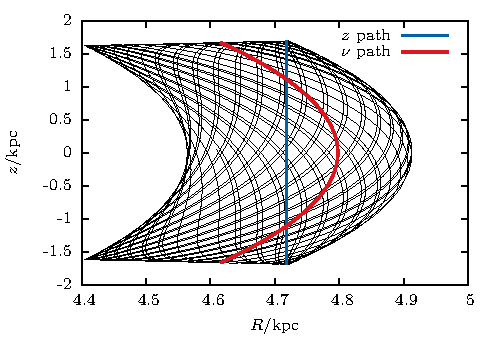
\includegraphics{{plots/SinglePoint.pdf}}$$
\caption[Difference between integration paths for the PAA and SAA]{Illustration of the difference between the PAA and SAA. An example orbit is shown by the black line. The blue line shows the line along which the PAA vertical-action integration is performed. The red line shows the line of constant $\lambda$ along which the SAA vertical-action integration is performed. The points at which they intersect gives the $(R,\pm|z|)$ coordinates of the input phase-space point.}
\label{SinglePoint}
\end{figure}

As we will see in Section~\ref{Sect::MethodComparison}, the SAA offers a considerable improvement over the PAA but unfortunately, due to the energy correction now being a function of three variables $(R,J_\phi,J_z)$, this approach takes slightly longer. However, the $E_\nu$ tabulation requires a very small number of $J_\phi$ values (here we use ten) over the required $J_\phi$ range for a sufficient level of accuracy. Note that the PAA is contained within the SAA. In the limit of very large focal distance, the surfaces of constant $\lambda$ and $\nu$ tend to those of constant $R$ and $z$. In this limit, the vertical action becomes independent of $J_\phi$ and the SAA tends to the PAA.

For our standard setup we use a linearly-spaced grid of $100$ points in $\lambda$, a linearly-spaced grid of $100$ points in $E_\nu^2$ and a $10$-point linearly-spaced grid in $L_z$.

\subsubsection{St\"ackel fudge}\label{Method::SF}
The SAA assumed the motion is separable in prolate spheroidal coordinates and we proposed 1D potentials that governed the motion in each coordinate. There are several ways of constructing approximate separable potentials from general axisymmetric and \cite{Binney2012} presented a method for constructing the approximate potential such that the equations of motion in a St\"ackel potential could be used. This approach was extended to the triaxial case by \cite{SandersBinney2015}. We begin by presenting the axisymmetric method in Section~\ref{Method::SF_Axi} and go on to present the triaxial method in Section~\ref{Method::SF_Triax}.
\paragraph{Axisymmetric case}\label{Method::SF_Axi}
\cite{Binney2012} presented a method for estimating the actions in a general axisymmetric potential by assuming it is close to a St\"ackel potential. For a general oblate axisymmetric potential, $\Phi$, we define
\begin{equation}
\begin{split}
\chi_\lambda(\lambda,\nu) &\equiv -(\lambda-\nu)\Phi,\\
\chi_\nu(\lambda,\nu) &\equiv (\lambda-\nu)\Phi.
\end{split}
\end{equation}
If $\Phi$ were a St\"ackel potential, these quantities would be given by
\begin{equation}
\begin{split}
\chi_\lambda(\lambda,\nu) &= F(\lambda)-F(\nu),\\
\chi_\nu(\lambda,\nu) &= F(\nu)-F(\lambda).
\end{split}
\end{equation}
Therefore, for a general potential we can write,
\begin{equation}
F(\tau) \approx \chi_\tau(\lambda,\nu)+D_\tau,
\end{equation}
where $D_\tau$ are constants provided we evaluate $\chi_\lambda$ at constant $\nu$ and vice versa. We can write the equations of motion (equation~\eqref{Eq::EqnOfMotionAxi}) as
\begin{equation}
2(\tau-a^2)(\tau-c^2)p_\tau^2 = E(\tau-c^2)-\Big(\frac{\tau-c^2}{\tau-a^2}\Big)\frac{J_\phi^2}{2}-B_\tau+\chi_\tau(\lambda,\nu),
\label{SFEqnOfMotion}
\end{equation}
where we have defined the integrals of motion $B_\tau = I_3-D_\tau$. Given an initial phase-space point, we use equation~\eqref{DeltaGuess} to find a suitable coordinate system, calculate $\lambda,\nu,p_\lambda$ and $p_\nu$, and use equation~\eqref{SFEqnOfMotion} to find the integrals $B_\tau$. Equation~\eqref{SFEqnOfMotion} is then integrated over an oscillation in $\tau$ to find the actions as in equation~\eqref{Eq::action}. We note that for the $\lambda$ integral we keep $\nu$ fixed at the input value, and vice versa.

\cite{Binney2014} presented an alternative method for estimating $\Delta$ based on the shell orbits ($J_R=0$). At each energy and $L_z$ a shell orbit is launched and an ellipse is fitted to the orbit in the meridional plane. The location of the focus of the ellipse give an estimate of $\Delta$. We will explore both methods for estimating $\Delta$ below.

\paragraph{Triaxial case}\label{Method::SF_Triax}
\cite{SandersBinney2015} presented a generalization of the above approach that is appropriate for estimating the actions in triaxial St\"ackel potentials. Given a general triaxial potential, we define the quantities
\begin{equation}
\begin{split}
\chi_\lambda(\lambda,\mu,\nu) &\equiv (\lambda-\mu)(\nu-\lambda)\Phi(\lambda,\mu,\nu),\\
\chi_\mu(\lambda,\mu,\nu) &\equiv (\mu-\nu)(\lambda-\mu)\Phi(\lambda,\mu,\nu),\\
\chi_\nu(\lambda,\mu,\nu) &\equiv (\nu-\lambda)(\mu-\nu)\Phi(\lambda,\mu,\nu).
\end{split}
\end{equation}
If $\Phi$ were a St\"ackel potential, these quantities would be given by, for instance,
\begin{equation}
\chi_\lambda(\lambda,\mu,\nu) = f(\lambda)-\lambda\frac{f(\mu)-f(\nu)}{\mu-\nu}+\frac{\nu f(\mu)-\mu f(\nu)}{\mu-\nu}.
\end{equation}
Therefore, for a general potential, we can write
\begin{equation}
f(\tau) \approx \chi_\tau(\lambda,\mu,\nu)+C_\tau\tau+D_\tau,
\end{equation}
where $C_\tau$ and $D_\tau$ are constants provided we always evaluate $\chi_\tau$ with two of the ellipsoidal coordinates fixed. For instance, we always evaluate $\chi_\lambda$ at fixed $\mu$ and $\nu$.

When we substitute these expressions into equation~\eqref{Eq::EqnOfMotion}, we find
\begin{equation}
2(\tau-a^2)(\tau-b^2)(\tau-c^2)p_\tau^2=\tau^2 E -\tau A_\tau+B_\tau +\chi_\tau(\lambda,\mu,\nu).
\label{Eq::EqnOfMotion_JK}
\end{equation}
For each $\tau$ coordinate, there are two new integrals of motion given by $A_\tau=a-C_\tau$ and $B_\tau=b+D_\tau$. Using a single 6D coordinate and a choice of coordinate system gives us a single constraint on a combination of $A_\tau$ $B_\tau$. Due to the separability of St\"ackel potentials the derivative of the Hamiltonian with respect to the ellipsoidal coordinates will be zero for a true St\"ackel potential. Setting it equal to zero for a general potential gives a further constraint on $A\tau$ and $B_\tau$ allowing us to solve for these integrals given only a single $(\bs{x},\bs{v})$ coordinate. We have therefore produced approximate $p_\tau(\tau)$ equations of motion which may be integrated to estimate the actions.

\subsubsection{St\"ackel fitting}\label{Method::FIT}
The above two methods used some approximate St\"ackel potential constructed from the target potential. An alternative procedure presented by \cite{Sanders2012a} is to explicitly fit a St\"ackel potential to the target potential and estimate the actions in a general axisymmetric potential. The method used the procedure from \cite{DejonghedeZeeuw1988} to find the locally best-fitting St\"ackel potential. This method seeks to minimise the difference between the target auxiliary function $(\lambda-\nu)\Phi$ and the St\"ackel auxiliary function $F(\nu)-F(\lambda)$. The best-fitting $F$ can be computed by an integral over a region of the prolate spheroidal coordinate system which can be defined on an orbit-by-orbit basis. We first integrate the orbit for several time-steps to form an average estimate of $\Delta^2$ via equation~\eqref{DeltaGuess}. We further integrate the orbit to determine the orbit boundaries in $\lambda$ and $\nu$. With the boundaries found we compute the best-fitting $F$ on a grid (we use $40$ grid points) and hence the best-fitting St\"ackel potential in which the actions can be computed as detailed in Section~\ref{StackelPot}.

The fitting procedure of \cite{DejonghedeZeeuw1988} uses weight functions which allow some flexibility in the fitting of the potential. We use weight functions $\Lambda(\lambda)\propto (\lambda-\Delta^2)^{-4}$ and $N(\nu)\propto (\nu-c^2)^0.5$.


\subsection{Convergent methods}\label{Sect::MethodsC}
All of the convergent methods detailed here are built on the construction of a generating function. Generating functions are mathematical objects for converting between sets of canonical coordinates. We saw in Section~\ref{Sect::analytic} the ease with which the actions can be analytically computed in a limited range of potentials (the isochrone and the harmonic oscillator). \cite{McGillBinney} exploited this idea to construct a generating function from the set of angle-actions $(\btheta,\boldsymbol{J})$ in one of these `toy' potentials to the set of angle-actions $(\btheta',\boldsymbol{J}')$ in the target potential. The generating function for the transformation is given by
\begin{equation}\label{eq:genGF}
S(\btheta,\bs{J}') = \btheta\cdot\bs{J}'
-2\i \sum_{\bs{n}>\bs{0}}S_{\bs{n}}(\bs{J}')\sin\bs{n}\cdot\btheta,
\end{equation}
where the vector $\bs{n}$ has integer components. The periodicity of the angle coordinates are used to express the generating function as a Fourier series with coefficients $S_{\bs{n}}$. The requirement of real actions has limited the Fourier series to just $\sin$ components. The sum over integer vectors $\bs{n}$ is limited to summing over half a 3D lattice by the time-reversible nature of the target Hamiltonians we consider. Using the properties of the generating function we find the toy actions are
\begin{equation}
\bs{J}=\frac{\partial S}{\partial \btheta} = \bs{J}'+2\sum_{\bs{n}>\bs{0}}\bs{n}S_{\bs{n}}(\bs{J}')\cos\bs{n}\cdot\btheta,
\label{toyact}
\end{equation}
and the target angles are
\begin{equation}
\btheta'=\frac{\partial S}{\partial \bs{J}'}
= \btheta+2\sum_{\bs{n}>\bs{0}}\frac{\partial S_{\bs{n}}}{\partial \bs{J}'}(\bs{J}')\sin\bs{n}\cdot\btheta.
\label{targetang}
\end{equation}
\cite{McGillBinney} constructed a algorithm that allowed for tori of given actions $\bs{J}'$ in an axisymmetric potential to be built. Points on the target torus are found by sampling in $\btheta$ and the corresponding toy actions $\bs{J}$ are found from equation~\eqref{toyact} assuming a set of $S_{\bs{n}}$. As the toy potential was chosen to be the isochrone the corresponding configuration space coordinates $(\bs{x}_i,\bs{v}_i)$ can be computed for each sample and in turn the energy, $E_i$. The $S_{\bs{n}}$ are iteratively adjusted until the spread in energy of the torus samples is minimised. \cite{KaasalainenB} demonstrated how this method could be applied in potentials that admitted different orbital families.

In order to find the derivatives of the Fourier coefficients $\partial S_{\bs{n}}/\partial \bs{J}'$, small sections of orbits are integrated starting from several points on the torus. Again, due to the simplicity of the toy potential the corresponding toy angles $\btheta$ can be computed for the orbital samples and the target angles $\btheta'$ are given by $\btheta'=\btheta'(0)+\boldsymbol{\Omega}'t$. We therefore have a series of linear equations that can be solved by standard methods.

\subsubsection{Iterative torus}\label{Method::ItTorus}
With the $S_{\bs{n}}$ and $\partial S_{\bs{n}}/\partial \bs{J}'$ found the corresponding $(\bs{x},\bs{v})$ for any point ($\btheta'$) on the torus ($\boldsymbol{J}'$) can be found. This is ideal for many applications but for others it is preferable to have machinery to convert $(\bs{x},\bs{v})$ to $(\btheta,\boldsymbol{J})$ \citep{McMillanBinney2013}. \cite{McMillanBinney2008} proposed an algorithm for repeatedly constructing tori to iteratively find the angle-action coordinates from $(\bs{x},\bs{v})$. However, the speed of this algorithm was limited by the quality of the initial guess. \cite{SandersBinney2015} proposed using a combination of one of the non-convergent methods with the torus machine.

\cite{SandersBinney2015} first estimated the angle-actions $(\btheta_S,\boldsymbol{J}_S)$ from $(\bs{x},\bs{v})$ using the axisymmetric St\"ackel fudge of \ref{Method::SF_Axi}. A torus with the corresponding actions $\boldsymbol{J}_S$ is constructed and the nearest configuration-space coordinate $(\bs{x}_S,\bs{v}_S)$ to $(\bs{x},\bs{v})$ is found by minimization with respect to the angle $\btheta$ using $\btheta_S$ as an initial guess. We then find an estimate of the angle-actions $(\btheta_P,\boldsymbol{J}_P)$ of the point $(\bs{x}_S,\bs{v}_S)$ from the the St\"ackel fudge and estimate the error in the actions produced by the St\"ackel fudge as $\Delta\boldsymbol{J}=\boldsymbol{J}_P-\boldsymbol{J}_S$. A better estimate to the action is then $\boldsymbol{J}_S-\Delta\boldsymbol{J}=2\boldsymbol{J}_S-\Delta\boldsymbol{J}_P$.

The procedure can be repeated using this improved action estimate to construct another torus. \cite{SandersBinney2015} found that a single torus construction produced actions accurate to $0.01\percent$ and further torus constructions only reduced this by a factor of two. For our standard setup we use $\eta=(0.1\kms)^2$, a maximum of $5$ torus constructions and a relative error for each torus construction of $\Delta J/J=1\times10^{-3}$. We integrate the orbits using an adaptive embedded Runge-Kutta Prince-Dortmund (8,9) scheme provided in the Gnu Science Library \citep{GSL} with a relative accuracy of $10^{-8}$.

\subsubsection{Generating function from orbit integration}\label{Method::Genfunc}
\cite{SandersBinney2014} discussed how the actions in a potential could be found using a very similar method to that employed in the torus machinery. The method operates by producing $N_\mathrm{samp}$ time samples from an orbit integrated for $N_T T$, where $T$ is the period of a circular orbit with the same energy. At each sample the actions and angles in a toy potential are computed. As with the angles we can use these toy angle-actions to construct a series of linear equations (equation~\ref{toyact}) and solving for the unknowns: the target actions and the Fourier coefficients, $S_{\bs{n}}$. We limit ourselves to vectors $\bs{n}<N_\mathrm{max}$.

In \cite{SandersBinney2014} the toy potential parameters were chosen by minimising the deviation of the toy Hamiltonian around the orbit. This procedure was computationally costly considering it was sub-optimal as it tended to produce very peaky variations of the Hamiltonian that required a large number of Fourier coefficients to remove. Here we find the minimum and maximum radius of the orbit sample and match the radial force of the toy potential. We only consider two toy parameters (the scale mass and radius of the isochrone) so this procedure is sufficient.

Several criteria for a sufficient sampling of toy angle space were discussed by \cite{SandersBinney2014}. For each vector $\bs{n}$ we compute the minimum and maximum $\bs{n}\cdot\btheta$ (where $\btheta$ are unrolled continuous angles i.e. not $2\pi$ periodic). If the difference between the minimum and maximum $\bs{n}\cdot\btheta$ is greater than $2\pi$ we repeat the algorithm with $N_T\rightarrow 2N_T$. Secondly if for any mode $\bs{n}\cdot\btheta/N_T>\pi$ the density of the sampling is too low to constrain the mode $\bs{n}$ and we repeat the algorithm with $N_\mathrm{samp}\rightarrow 2N_\mathrm{samp}$. For our standard setup we use $N_T=8$, $N_\mathrm{samp}=300$ and $N_{\rm max}=8$, and integrate the orbits using an adaptive embedded Runge-Kutta Prince-Dortmund (8,9) scheme provided in the Gnu Science Library \citep{GSL} with a relative accuracy of $10^{-8}$.

\cite{SandersBinney2014} showed how the actions could be found in a triaxial potential where there are several orbital families. In this case one must choose an appropriate toy potential to match the orbit class. This was determined by checking whether the sign of the angular momentum components changed over the orbit. If so, a triaxial harmonic oscillator is appropriate as the toy potential and if not the isochrone potential is suitable.


\subsubsection{Averaging toy actions over toy angles}\label{Method::AvGenfunc}
As noted by \cite{Bovy2014} and \cite{Fox2014} if one averages equation¬\eqref{toyact} over the toy angles one yields an expression for the target actions:
\begin{equation}
\bs{J}'=\int\mathrm{d}^3\btheta\Big(\boldsymbol{J}-2\sum_{\bs{n}>\bs{0}}\bs{n}S_{\bs{n}}(\bs{J}')\cos\bs{n}\cdot\btheta\Big)=\int\mathrm{d}^3\btheta\,\boldsymbol{J}.
\end{equation}
 Such an approach is suitable when one has a good coverage in the toy angle coordinates and speeds up the computation as one avoids solving a matrix equation. For the standard setup we use the same parameters as for the generating function method.

\section{Method comparison}\label{Sect::MethodComparison}
In this section we present a critical comparison of the methods presented above. We are interested in two quantities for each method: the accuracy of the action computation (i.e. how constant are the actions around an orbit) and how much computing time is required. The latter of these quantities is slightly subjective as it varies on precise implementation and computational details. However, we will see that the time differences between the methods are orders of magnitude such that even with improved implementations we expect the hierarchy to be maintained.

We limit our comparison to the axisymmetric versions of the described algorithms. This is because there are more competing methods for the axisymmetric case. In the triaxial case the choice currently is between using the generating function method of Section~\ref{Method::Genfunc} if one requires a few accurate actions and the St\"ackel fudge method of Section~\ref{Method::SF_Triax} if one requires many actions with a lower level of accuracy. The list of axisymmetric methods we will compare are
\begin{enumerate}
\item Polar adiabatic approximation (PAA), Section~\ref{Method::PAA}
\item Spheroidal adiabatic approximation (SAA), Section~\ref{Method::SAA}
\item St\"ackel fudge with $\Delta$ chosen using equation~\eqref{DeltaGuess} (Fudge v1), Section~\ref{Method::SF}
\item St\"ackel fudge with $\Delta$ chosen from shell orbits (Fudge v2), Section~\ref{Method::SF}
\item Locally fitting St\"ackel potentials (Fit), Section~\ref{Method::FIT}
\item Iterative torus construction (ItTorus), Section~\ref{Method::ItTorus}
\item Averaging toy actions over toy angles (AvGenfunc), Section~\ref{Method::AvGenfunc}
\item Finding Fourier coefficients from orbit (Genfunc), Section~\ref{Method::Genfunc}
\end{enumerate}
We begin by inspecting the actions computed for a series of time samples from single orbits in Section~\ref{SingleOrbs} and we go on to investigate the action, angle and frequency variances for a broader range of orbits in Section~\ref{ManyOrbs}.

\subsection{Single orbits}\label{SingleOrbs}

\begin{figure*}
\centering
\begin{minipage}{.5\textwidth}
\centering
$$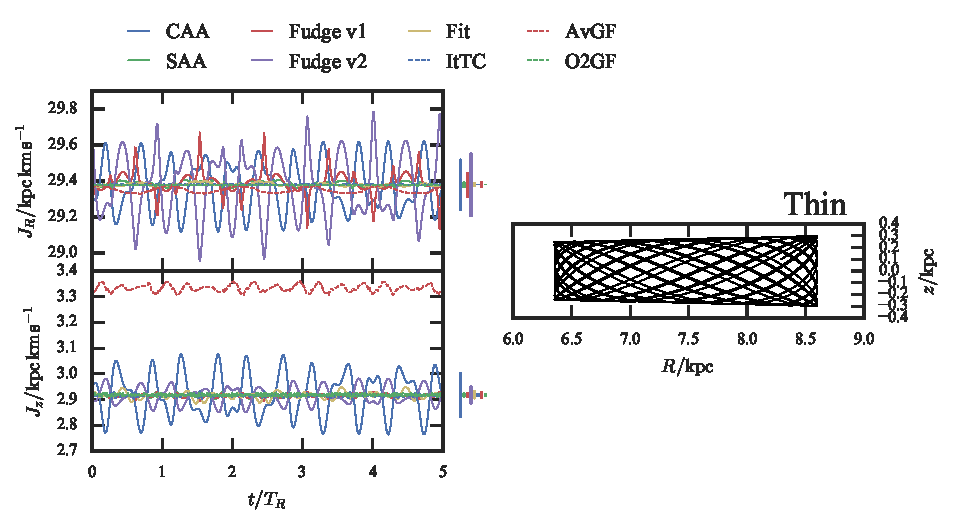
\includegraphics[width=\textwidth]{{{plots/thin.action}}}$$
\end{minipage}%
\begin{minipage}{0.5\textwidth}
\centering
$$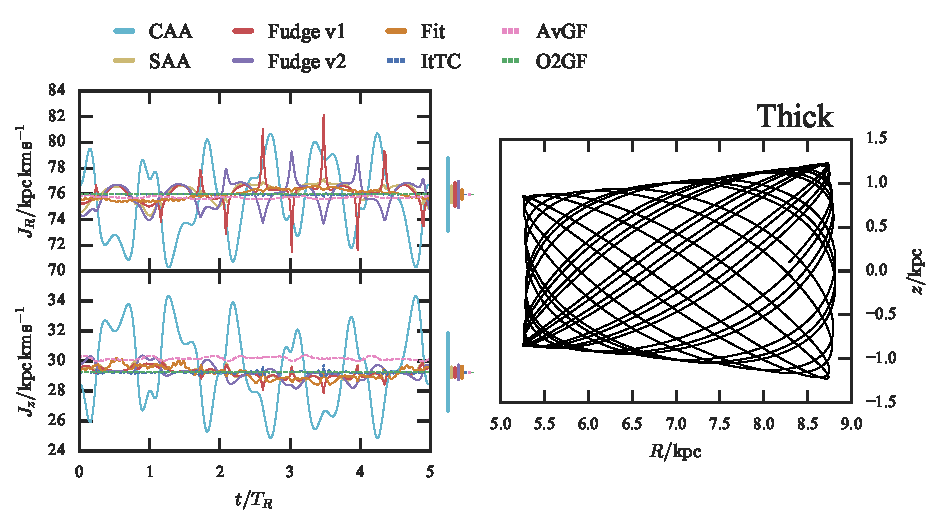
\includegraphics[width=\textwidth]{{{plots/thick.action}}}$$
\end{minipage}
\begin{minipage}{.5\textwidth}
\centering
$$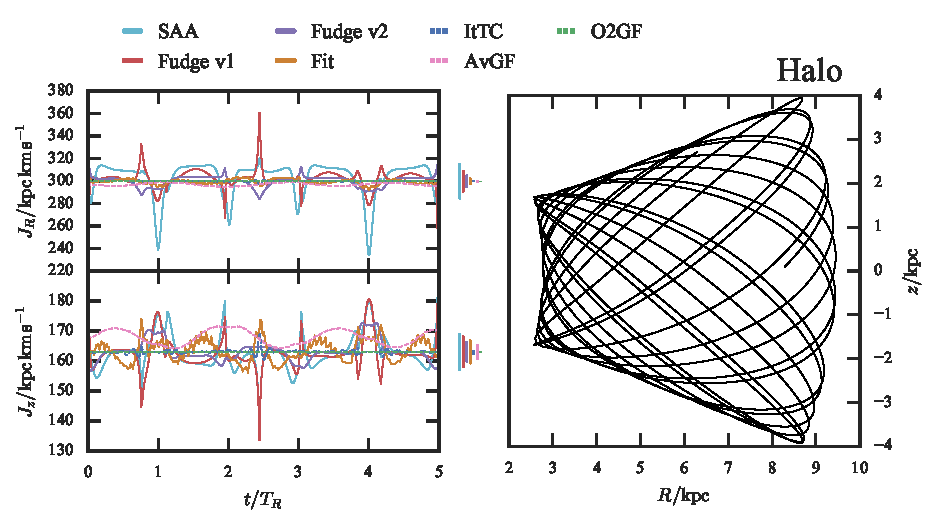
\includegraphics[width=\columnwidth]{{{plots/halo.action}}}$$
\end{minipage}%
\begin{minipage}{0.5\textwidth}
\centering
$$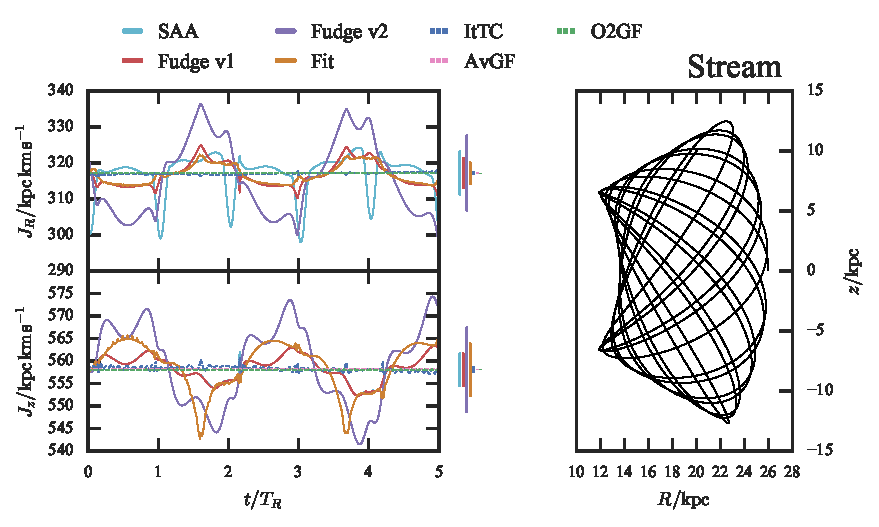
\includegraphics[width=\columnwidth]{{{plots/stream.action}}}$$
\end{minipage}
\caption{Comparison of action estimation methods for single orbits. The top left set of panels corresponds to a typical \emph{thin} disc orbit, top right a typical \emph{thick} disc orbit, bottom left a typical \emph{halo} orbit and bottom right a typical orbit for the progenitor of a tidal \emph{stream}. Each set of panels shows the radial action, $J_R$, (top left panel) and the vertical action, $J_z$, (bottom left panel) computed as a function of number of radial periods for the different methods. The \emph{non-convergent} methods are shown with solid lines whilst the \emph{convergent} methods are shown with dashed lines. Blue solid corresponds to the polar adiabatic approximation, green solid the spheroidal adiabatic approximation, red solid the St\"ackel fudge with variable $\Delta$ estimation, purple solid the St\"ackel fudge with $\Delta$ estimation from shell orbits, solid mustard yellow the St\"ackel fitting method, blue dashed the iterative torus method, green dashed the generating function method and red dashed the averaging method. To the left of each panel the vertical lines show the $\pm$ standard deviation spread in the action estimates from each method. In each set of panels the orbit in the meridional plane $(R,z)$ is shown on the right. All orbits are computed in the multi-component potential from \protect\cite{Piffl2014}.}
\label{Fig::SingleOrbs}
\end{figure*}


\begin{table*}
\caption{Action errors for four example orbits: On the first line we give the radial and vertical actions for the four orbits in units of $\kpc\kms$. Below the double horizontal separators we give the standard deviations of the radial and vertical action estimates for the $7$ methods. The methods above the horizontal separator are the non-convergent methods whilst those below are the convergent methods.}
\begin{tabular}{llrrrrrrrr}
% \hline
&&\multicolumn{2}{c}{Thin}&\multicolumn{2}{c}{Thick}&\multicolumn{2}{c}{Halo}&\multicolumn{2}{c}{Stream}\\
&&$J_R$&$J_z$&$J_R$&$J_z$&$J_R$&$J_z$&$J_R$&$J_z$\\
\hline
 &Actions & 29.38 & 2.92 & 75.96 & 29.25 & 299.79 &  163.02 & 317.20 &   558.09 \\
\hline
\hline
 \textbf{Method}&CAA      & 0.1   & 0.08  & 3   & 3   & 40 & 50 & 100 & 200 \\
 &SAA      & 0.01  & 0.007 & 0.7 & 0.4 & 10 & 6     & 6     & 4     \\
 &Fudge v1 & 0.07  & 0.007 & 1   & 0.3 & 9     & 5     & 4     & 3     \\
 &Fudge v2 & 0.2   & 0.03  & 1   & 0.5 & 5     & 3     & 10 & 9     \\
 &Fit      & 0.007 & 0.01  & 0.4 & 0.4 & 2     & 4     & 3     & 6     \\
\hline
 &ItTC   & 0.002  & 0.008 & 0.03  & 0.06  & 0.3  & 0.8  & 0.4  & 0.6  \\
 &AvGF & 0.03   & 0.4   & 0.2   & 2     & 3    & 6    & 0.2  & 0.3  \\
 &O2GF   & 0.0003 & 0.005 & 0.002 & 0.007 & 0.03 & 0.03 & 0.01 & 0.01 \\
\hline
\end{tabular}

\label{Table}
\end{table*}

We inspect how the actions vary along orbits when computed using the variety of methods in Section~\ref{Methods}. We choose to analyse the results for four different orbits that reflect the range of interesting orbits one wishes to explore when constructing models for the Galaxy. We select a typical \emph{thin} disc orbit, a typical \emph{thick} disc orbit, a typical \emph{halo} orbit and a typical orbit for the progenitor of a tidal \emph{stream}. The initial conditions for the four orbits chosen are:
\begin{enumerate}
\item Thin, $\bs{x} = (8.29,0.1,0.1)\kpc, \bs{v}=(30.22,211.1,19.22)\kms$,
\item Thick, $\bs{x} = (8.29,0.1,0.1)\kpc, \bs{v}=(50.22,187.1,54.22)\kms$,
\item Halo, $\bs{x} = (8.29,0.1,0.1)\kpc, \bs{v}=(100.22,109.1,101.22)\kms$,
\item Stream, $\bs{x} = (26.,0.1,0.1)\kpc, \bs{v}=(0.1,141.8,83.1)\kms$.
\end{enumerate}
The thin, thick and halo orbits were chosen arbitrarily but the stream orbit is selected as a likely orbit for the progenitor of the GD-1 stream \citep{Koposov2010,SandersBinney2013b}. Each orbit was integrated for $10$ orbital periods of a circular orbit of the same energy and $1000$ time samples were recorded. We chose to integrate the orbits in the multi-component Galactic potential from \cite{Piffl2014}. This potential was fitted to the RAVE data as well as other potential constraints from \cite{McMillan2011} and consists of three exponential discs (thin, thick and gas), a central bulge and an NFW dark halo. The actions were computed using the $8$ different methods for each time sample and the resulting estimates are plotted in Fig.~\ref{Fig::SingleOrbs} and shown in Table~\ref{Table}. We will discuss in detail the results for each method. The iterative torus method and generating function method produce RMS deviations that are small enough for all purposes for all the inspected orbits so we will not comment on them further in this section.


\subsubsection{Thin}
From the plot of the orbit in the meridional plane we can clearly see that the orbit is near separable in cylindrical polar coordinates. However, the St\"ackel fudge method and the SAA give better results than the PAA. Of the non-convergent method St\"ackel fitting gives the most accurate results.

For this very low eccentricity orbit locally choosing $\Delta$ around the orbit (Fudge v1) gives better results than using the closed orbits (Fudge v2) but this is probably due to the grid used to compute $\Delta$ for the closed orbits.

The averaging method gives slightly biased estimates in both the radial and vertical action. One reason for this is because the toy actions are always positive so for small actions averaging produces a positively biased action. This can be improved by using a better toy potential but we do not explore this here.

\subsubsection{Thick}
For the thick disc orbit we begin to see more curvature of the boundaries of the orbit such that the assumption of separability in cylindrical polar coordinates is clearly breaking down. For this reason the polar adiabatic approximation is noticeably inferior to the other methods by a factor of a few. All four of the methods based on St\"ackel potentials give comparable accuracy for $J_z$ but the St\"ackel fitting gives a factor of two more accurate result than the other methods for $J_R$. As with the thin-disc orbit the averaging method gives a slightly biased estimate for both $J_R$ and $J_z$ with the error in $J_z\sim 1\kpc\kms$.
\subsubsection{Halo}
For the halo and stream orbits we have not plotted the polar adiabatic approximation result as it is not competitive at these higher eccentricities. The hierarchy for the St\"ackel-type methods is SAA, Fudge v1, Fudge v2 and St\"ackel-fitting with the St\"ackel-fitting method producing a factor of five more accurate result than the SAA for $J_R$ but all three produce equally accurate results for $J_z$. Again we note there is a small systematic shift in $J_z$ for the averaging method.
\subsubsection{Stream}
Finally, the stream-like orbit has a similar hierarchy for the St\"ackel-type methods. Both the St\"ackel fudge v1 and SAA produce very similar results for both $J_R$ and $J_z$. St\"ackel-fitting produces more accurate results for $J_R$ but less accurate for $J_z$ and the St\"ackel fudge v2 produces slightly larger errors in both $J_R$ and $J_z$. Clearly an estimate for $\Delta$ based on a shell orbit is not optimal for this more radially-extended orbit. There are no obvious systematic shifts in the actions from the averaging method.

\subsection{Convergence of the generating function method}
In the previous section we highlighted the difference between the convergent and non-convergent methods. For the presented orbits we have shown the errors in the actions computed from the convergent methods using a single set of parameters. Here we briefly show how the error in the actions changes as a function of the parameters in the generating function method.

There are three parameters to choose for the generating function method: the integration time $N_T$, the number of samples $N_\mathrm{samp}$ and the number of Fourier coefficients (controlled by the parameter $N_\mathrm{max}$). From investigation we found that the error in the action was most strongly a function of the number of Fourier coefficients. For the frequencies and angles the error is also affected by the total integration time.

In Fig.~\ref{Fig::Genfunc_converg} we show the error in the actions for the four orbits considered in this section as a function of $N_\mathrm{max}$ and computation time using fixed $N_T=24$ and $N_\mathrm{samp}=2400$. In general, we see that as required the error decreases as a function of $N_\mathrm{max}$ and more Fourier coefficients takes more time. There are a few cases where the error rises as a function of $N_\mathrm{max}$ as we have introduced Fourier coefficients which make the situation worse and must be cancelled by higher order coefficients. We see that for small $N_\mathrm{max}$ the computation time is dominated by the orbit integration and the thin-like orbit is much easier to integrate than the halo-like. However, at large times the computational budget is dominated by the large number of $N_\mathrm{max}$ so each orbit takes a similar time. For the largest $N_\mathrm{max}$ the stream-like orbit takes slightly longer as the algorithm has decided to integrate the orbit longer to achieve a better sampling density in toy angles.

\begin{figure}
$$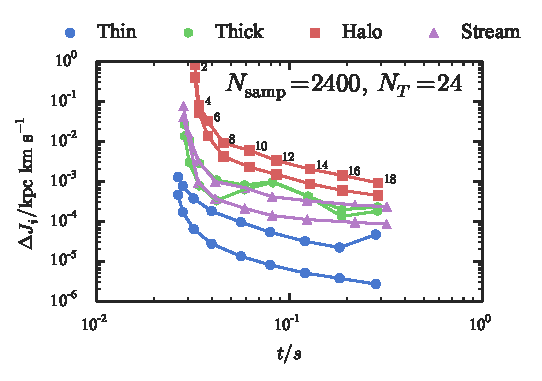
\includegraphics[width=\columnwidth]{{{plots/genfunc_converg}}}$$
\caption{Error in the actions as a function of computation time for the generating function method using different numbers of Fourier coefficients: $N_\mathrm{max}$ is the maximum magnitude of the Fourier vectors $\bs{n}$ considered. We show the radial (bottom for all) and vertical action errors for thin- (blue circles), thick- (green hexagons), halo- (red squares) and stream-like (purple triangles) orbits. The halo points are labelled by $N_\mathrm{max}$. For all cases we fix $N_T=24$ and $N_\mathrm{samp}=2400$.}
\label{Fig::Genfunc_converg}
\end{figure}

\subsection{Multiple orbits}\label{ManyOrbs}
We now go on to inspect a more extended sample of orbits. Each orbit has $J_\phi=R_0V_c(R_0)$ where $R_0$ is the solar radius and have increasing energy. For each energy we set $v_z=0.8v_R$ and launch the orbit from the solar position. We integrate the orbits for $10$ periods of the circular orbit with the same energy and store $40$ points in the orbit integration. As in the previous section the orbits were integrated using the embedded Runge-Kutta Prince-Dortmund (8,9) scheme provided in the Gnu Science Library \citep{GSL} with a relative accuracy of $10^{-8}$. The most extreme orbit considered has pericentre $\sim5\kpc$, apocentre $\sim28\kpc$ and maximum Galactic height $\sim15\kpc$.

\subsubsection{Action accuracy}
In Figure~\ref{MultiOrbits} we show the RMS action deviations away from the mean of the generating function method using each method for the described range of orbits.

In the previous section we discussed the relative merits of the various methods. We did not touch on the question of how accurate the actions \emph{need} to be. When constructing dynamical models we are perhaps less concerned with the absolute accuracy of the actions and more concerned with the accuracy of the corresponding probability of the action, or even integrated moments of the probability such as the density or the velocity dispersion. \cite{BinneyMcMillan2011} compared the recovery of the velocity distributions and the density profile for action-based disc models computed using the adiabatic approximation with those computed using tori and found that below a Galactic height of $1\kpc$ the differences were very small whilst above this the adiabatic approximation produced results that are in error by $\sim10\percent$. Similarly, \cite{BovyRix2013} showed a comparison between the adiabatic approximation and the St\"ackel fudge. They found that the difference in the vertical velocity dispersion for a near-flat profile was $\sim1\percent$ in error. \cite{SandersBinney2014} demonstrated that the action estimates from the triaxial St\"ackel fudge method are accurate enough to satisfy the Jeans' equations for a triaxial Navarro-Frenk-White halo profile. These studies demonstrate that although the error in the actions for individual orbits can be large for some methods, the resulting moments of the distribution function are well recovered as they are presumably dominated by those low-action orbits that have good action estimates.

In Appendix~\ref{Appendix} we give details of four distribution functions that describe components of the Galaxy. With these distribution functions we are able to compare the accuracy of the action calculation required to resolve the distribution functions to a certain accuracy. In Figure~\ref{MultiOrbits} we show four coloured bands. The three labelled \emph{thin}, \emph{thick} and \emph{halo} give the accuracy required to calculate the corresponding distribution function to between $1$ and $10\percent$. The band labelled stream shows the action-space spreads for a stream created from a progenitor with a velocity dispersion of between $0.5$ and $5\kms$.

MORE DISCUSSION

RESONANT LINES

We have also inspected a series of orbits parented by the circular orbit at $5\kpc$ and at $13\kpc$. The hierarchy of the action accuracy is very similar to the $8\kpc$ case with general the order of increasing accuracy being: Genfunc, ItTorus, AvGenfunc, Fit, Fudge, SAA, PAA. We also tested the methods in a flattened logarithmic potential ($q=0.9$). The errors with the actions are much smoother in this case and no clear resonances are visible. The magnitude of the errors in the actions are very similar to those in the more complex potential. Also, the St\"ackel fitting procedure seems to perform slightly worse. The generating function method produces significantly smaller errors ($\sim$ a factor of ten) as the smoothness of the potential means fewer terms in the generating function are required.

\subsubsection{Computational time}
In Figure~\ref{MultiOrbits_Time} we show the average time for computing a single action for each method. The most computationally efficient method is the St\"ackel fudge method. With our setup each action takes $\sim10^{-5}\mathrm{s}$ but note that speed-ups are possible as the accuracy of the root-finding and Gauss-Legendre integration can be adjusted. The adiabatic approximations take two to three times longer than the St\"ackel fudge as for each action integrand call we must perform a linear interpolation in $2$ variables for the PAA and $3$ for the SAA (hence the SAA taking slightly longer). Of the non-convergent methods the St\"ackel-fitting method takes the longest and shows a factor of three increase in computational time over the range of actions explored. This is the only non-convergent method that requires orbit integration and again the accuracy of the orbit integration or the integration routine can be tuned to the given problem to achieve speed-ups.

The averaging method is the fastest of the three convergent methods as it only requires an orbit integration. The generating function method is a factor of three slower as we require an additional matrix solve. The jagged nature of the line is because the routine has chosen for certain orbits to integrate for longer to get better coverage in some modes. The iterative torus method is a factor of ten slower again. Each torus construction is the equivalent of two matrix solves (one for the $S_{\bs{n}}$ and another for the derivatives) and we have allowed a maximum of five torus constructions. Binney \& McMillan (2015, in prep.) have provided details of how one could interpolate tori to allow for considerable speed-ups using this method.

\begin{figure}
$$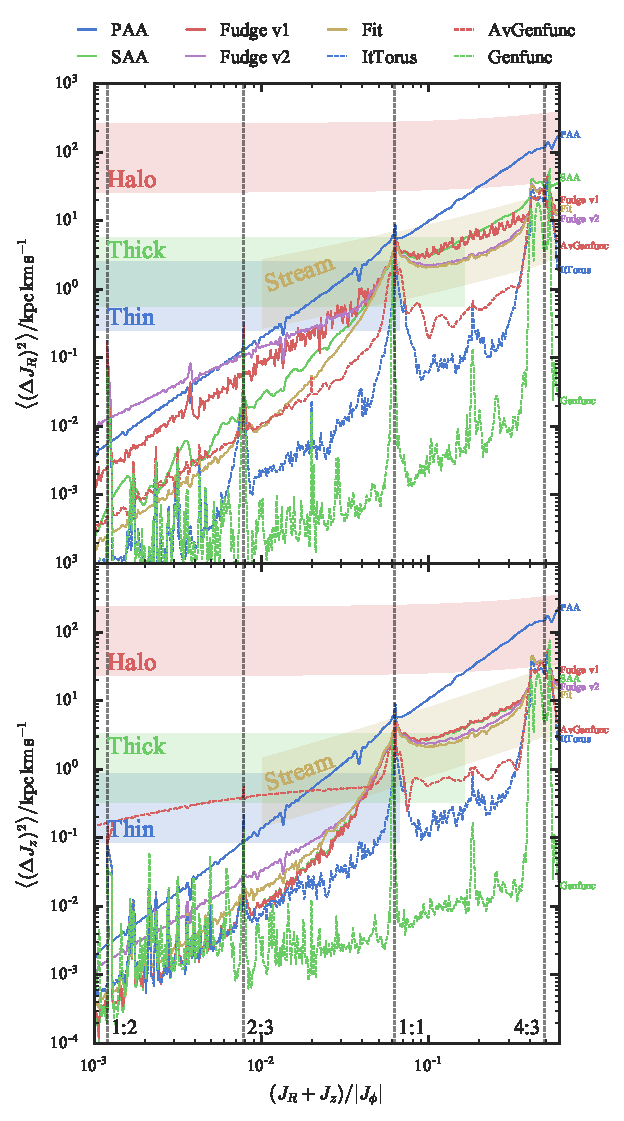
\includegraphics[width=\columnwidth]{{{plots/many_tori_output.dat.acc}}}$$
\caption{Comparison of the accuracy of the action-estimation methods for multiple orbits: each panel shows the root-mean-squared deviations of the estimates from the mean computed using the generating function method. The top panel shows the radial action $J_R$ and the bottom panel shows the vertical action $J_z$. The \emph{non-convergent} methods are shown with solid lines whilst the \emph{convergent} methods are shown with dashed lines. Blue solid corresponds to the polar adiabatic approximation, green solid the spheroidal adiabatic approximation, red solid the St\"ackel fudge with variable $\Delta$ estimation, purple solid the St\"ackel fudge with $\Delta$ estimation from shell orbits, solid mustard yellow the St\"ackel fitting method, blue dashed the iterative torus method, green dashed the generating function method and red dashed the averaging method. The coloured bands show the region in which the relative error in the action-based distribution functions for the thin (red), thick (green) and halo (red) components are between $1$ and $10\percent$. The upper and lower boundaries of the yellow band correspond to the action-space widths of streams with velocity dispersions of $5$ and $0.5\kms$. The chosen horizontal limits of these bands are $\log f/f_{\rm max}=-5$ for the thin and thick components and $(J_R+J_z)/|J_\phi|=0.01$ for the stream component. The vertical grey dashed lines correspond to resonances $x:y$ when $\Omega_R/\Omega_z=x/y$.}
\label{MultiOrbits}
\end{figure}

\begin{figure}
$$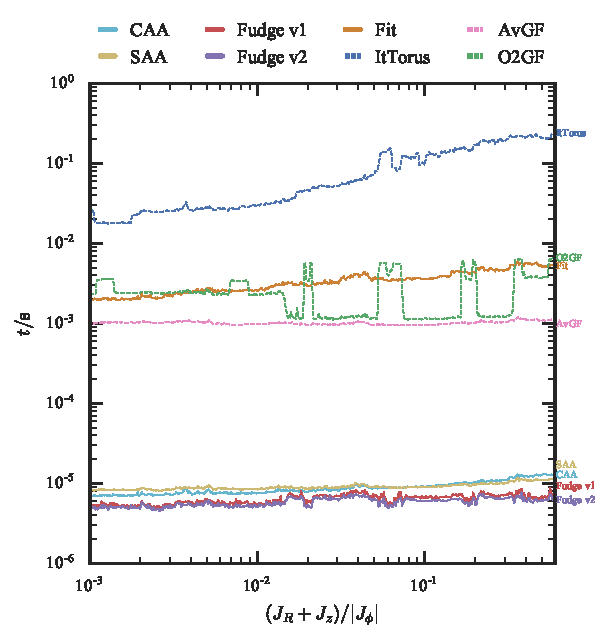
\includegraphics[width=\columnwidth]{{{plots/many_tori_output.dat.times}}}$$
\caption{Comparison of the speed of the action-estimation methods for multiple orbits. The colour-coding and range of orbits explored are as in \protect\ref{MultiOrbits}. The time quoted is the time per action estimation averaged from $50$ estimates per orbit.}
\label{MultiOrbits_Time}
\end{figure}


\section{Angle and frequency estimation}\label{Sect::AngleFreq}

We close this review by comparing the accuracy with which the angle and frequency coordinates are estimated using the presented methods. The angle coordinates are related to the generating function, $S$, as
\begin{equation}
\btheta = \frac{\partial S}{\partial \bs{J}}.
\end{equation}
In a separable cylindrical potential this generating function is given by
\begin{equation}
S(R,\phi,z,J_R,J_\phi,J_z) = \int_{}^R\mathrm{d}R\,p_R+\int_{}^\phi\mathrm{d}\phi\,p_\phi+\int_{}^z\mathrm{d}z\,p_z.
\end{equation}
In a potential separable in spheroidal coordinates this expression is altered by changing the integrals over the $R$ and $z$ momenta by those over $\lambda$ and $\nu$ momenta.
The angle coordinates can be computed by writing
\begin{equation}
\theta_i = \sum_k\frac{\partial S}{\partial I_k}\frac{\partial I_k}{\partial J_i}.
\end{equation}
For separable potentials, the first term is computed by differentiating the momenta $p_i$ with respect to the classical integrals $\bs{I}$ and integrating along the coordinate path. The second term is computed by inverting the matrix $\partial \bs{J}/\partial \bs{I}$ which again is found by differentiating the momenta in the action integrals and integrating over the full orbital path (see for example the appendix of \cite{Sanders2012a}). This approach can be extended to compute the angles using the presented approximation schemes. In the adiabatic approximations the three integrals are taken to be $(E,J_\phi,J_z)$. When computing the derivatives of the generating function and $J_R$ with respect to $J_z$ we require the derivatives $\partial J_z/\partial E_z|_R$ and $\partial J_z/\partial E_\nu|_{\lambda,J_\phi}$ which must be computed from the grids. In the St\"ackel fudge the classical integrals are $(E,J_\phi,B_\tau)$ and finally in the St\"ackel fitting procedure the classical integrals are those in any St\"ackel potential i.e. $(E,J_\phi,I_3)$. The frequencies are given by $\partial H/\partial \bs{J}$ and so are just single components of the inverted $\partial \bs{J}/\partial \bs{I}$ matrix.

For these approximate methods it is worth considering the difference between computing the actions and the frequency variables. The actions are the integral of the momenta whilst the frequencies are the integral of the inverse of the momenta. Therefore, the error in the action is dominated by the high momenta regions of the orbit whilst the error in the frequency is dominated by the momenta near the turning points. For this reason, the frequency estimation is much more sensitive to the location of the turning points whilst the action estimation is more sensitive to how closely the potential is mapped in the body of the orbit.

For the generating function method the angles are computed by solving for the derivatives of the Fourier components as discussed in Section~\ref{Method::Genfunc} and for the iterative torus approach the angles are computed from an angle fit of the final torus.

\subsection{Multiple Orbits}
In Figures~\ref{MultiOrbits_Freq} we show the RMS deviations of the frequencies away from the mean of the generating function method and in Figure~\ref{MultiOrbitsAng} we show the RMS deviation of the angles from those computed with the generating function method. The yellow band shows the width in frequencies and angles of particles very recently stripped from a progenitor with a velocity dispersion between $0.5$ and $5\kms$. Note that the spread in the angles grows in time as the stream grows so the given width is the smallest one would ever wish to resolve.

\begin{figure}
$$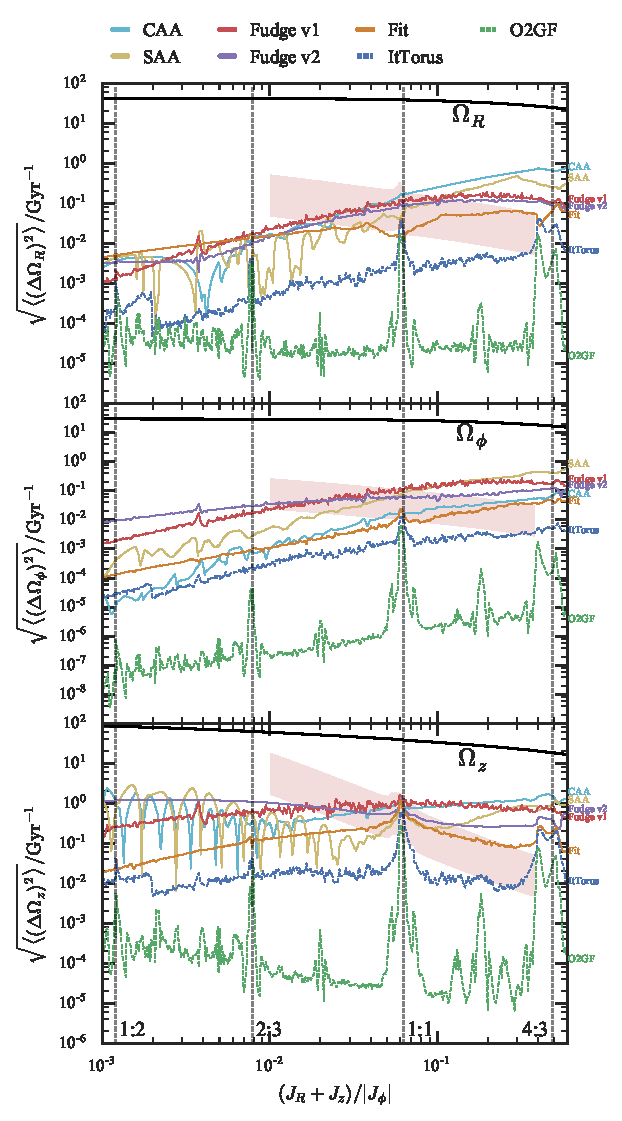
\includegraphics[width=\columnwidth]{{{plots/many_tori_output.dat.freq}}}$$
\caption{Comparison of the accuracy of frequency estimation using different methods for multiple orbits: the top panel shows the radial frequency, middle panel the azimuthal and bottom the vertical. The colour-coding and range of orbits explored are as in \protect\ref{MultiOrbits}. The upper and lower boundaries of the yellow band correspond to the frequency widths of streams with velocity dispersions of $5$ and $0.5\kms$. The vertical grey dashed lines correspond to resonances $x:y$ when $\Omega_R/\Omega_z=x/y$.}
\label{MultiOrbits_Freq}
\end{figure}
\begin{figure}
$$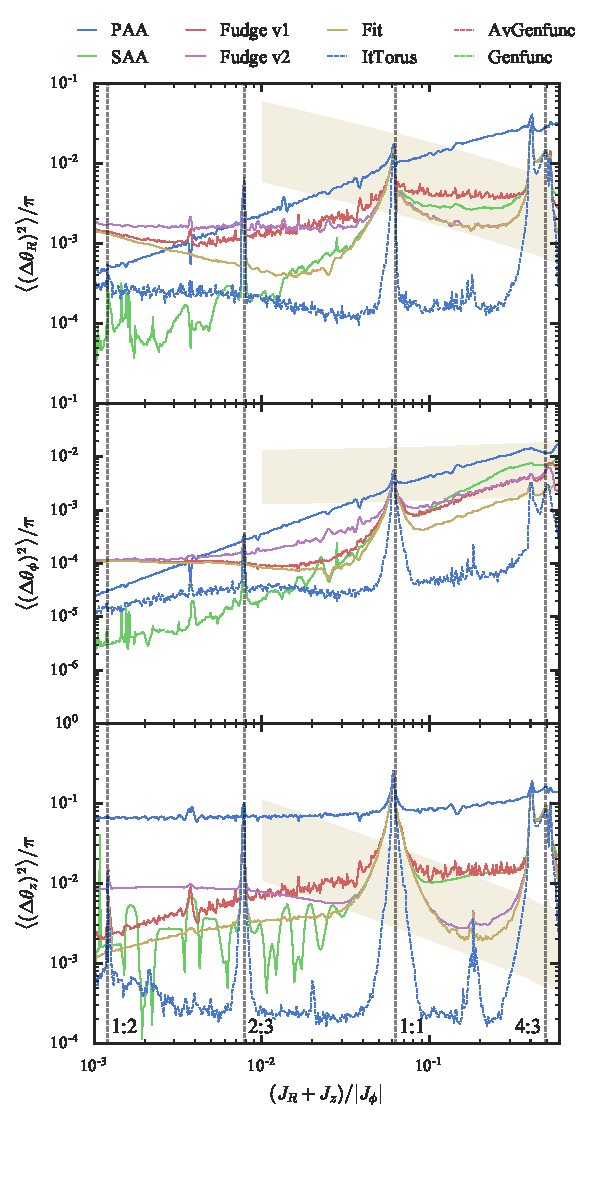
\includegraphics[width=\columnwidth]{{{plots/many_tori_output.dat.ang}}}$$
\caption{Comparison of the accuracy of angle estimation using different methods for multiple orbits: the top panel shows the radial angle, middle panel the azimuthal and bottom the vertical. The colour-coding and the range of orbits explored are as in \protect\ref{MultiOrbits}. The upper and lower boundaries of the yellow band correspond to the angle widths of streams with scale radii of $100$ and $10\pc$. The vertical grey dashed lines correspond to resonances $x:y$ when $\Omega_R/\Omega_z=x/y$.}
\label{MultiOrbitsAng}
\end{figure}
\section{Conclusions}\label{Sect::Conclusions}
We have presented a review of the currently available algorithms for estimating actions, angles and frequencies in general potentials. We focussed on axisymmetric potentials with the emphasis being on action estimation in the Milky Way. The presented methods fall into two groups: non-convergent methods and convergent methods.

The non-convergent methods are based on the cases for which we can compute the actions can be expressed as one-dimensional quadratures i.e. the St\"ackel potentials. These methods assume the potential is sufficiently close to one of these separable cases and the associated accuracy of the action computation is only as good as the approximation. The convergent methods, on the other hand, are designed to produce ever more accurate action estimates given increased computation times. These methods are entirely complementary. For some applications one requires a few accurate action computations (e.g. stream modelling) whilst for other applications one requires many less accurate actions (e.g. disc or halo modelling).

We began by comparing the action estimation for four example orbits in a multi-component axisymmetric Galactic potential and discussed the accuracy of the action computation from each method for each orbit. We went on to compare the accuracy of the actions for a series of orbits in the same potential and also discussed the computational speed of each method. We closed with a discussion of the accuracy of the angle and frequency computation.

We have seen the effect of resonant orbits on the methods. For resonant orbits one action describes the oscillation about the resonance. Many of the non-convergent methods lack the ability to identify a resonance and the associated action estimates are for the closest integrable Hamiltonian which oscillates significantly. If one wishes to handle the resonances specifically one must use the convergent methods and the torus machine whilst carefully choosing the toy potential to match the nature of the resonance (\cite{KaasalainenB}, Binney \& McMillan 2015).

\subsection{\texttt{tact} Code}
`The Action Computation Tool' or \texttt{tact} is a publicly-available code implementing all the algorithms given in this paper and is available at \href{https://github.com/jls713/tact}{https://github.com/jls713/tact}. We also provide programs to produce the plots given in this paper, and there is documentation describing each of the algorithms. The code is implemented in C++ but there is code available to compile the routines into a Python library. The code can work in tandem with \texttt{TTC} (the Torus code) that is described by Binney \& McMillan (2015, in prep.).

Each algorithm discussed in the paper is implemented by an \texttt{Action\_Finder} class. These classes take a potential class (\texttt{Potential\_JS}) and all have routines \texttt{actions} and \texttt{angles} that return the actions, and angles and frequencies given some Cartesian 6D phase-space point $(x,y,z,v_x,v_y,v_z)$. It should be simple for users to specify their own potential by implementing an inherited class of \texttt{Potential\_JS} and specifying a function for the potential \texttt{Phi} and the forces \texttt{Forces}. We also provide a simple \texttt{Orbit} class that may be used with custom potentials.

\section*{Acknowledgments}
We thank Angus Williams for constructing the backronym `The Action Computation Tool' for the \texttt{tact} code.

\bibliography{bibliography}
\bibliographystyle{mn2e}

\appendix
\section{Relative errors in distribution functions for Galactic components}\label{Appendix}
\subsection{Thin and thick discs}
For both the thin and thick discs we use the quasi-isothermal distribution function presented in \cite{Binney2010}. This distribution function is nearly-separable in the actions such that the radial and vertical dependence is given by
\begin{equation}
f_\mathrm{disc}(J_R,J_z) \propto \exp \Big(-\frac{\kappa J_R}{\sigma_R^2}-\frac{\nu J_z}{\sigma_z^2}\Big),
\end{equation}
where $\kappa$ and $\nu$ are the epicyclic frequencies and $\sigma_R$ and $\sigma_z$ are velocity dispersion parameters. We adopt the parameter values from \cite{Piffl2014} that were found to produce a good fit to the RAVE data. From a distribution function of this form the relative error in the distribution function is given by
\begin{equation}
\Big(\frac{\Delta f_\mathrm{disc}}{f_\mathrm{disc}}\Big)^2 = \sqrt{\Big(\frac{\kappa\Delta J_R}{\sigma_R^2}\Big)^2+\Big(\frac{\nu\Delta J_z}{\sigma_z^2}\Big)^2}.
\end{equation}
Note that due to the form of the distribution function the relative error in the distribution function is independent of the actions.

\subsection{Stellar halo}
For the stellar halo we use the distribution function from \cite{Williams2015}. This distribution function was fitted to the Blue Horizontal Branch stars from the SEGUE survey and has the form
\begin{equation}
f_\mathrm{halo}\propto \mathcal{L}^{-q}(\mathcal{L}^2+J_b^2)^{-(p-q)/2},
\end{equation}
where
\begin{equation}
\mathcal{L} = \mathcal{F}D_0 J_R+|J_\phi|+J_z.
\end{equation}
$p=0.83$ and $q=9.16$ govern the inner and outer slopes of the density profile and $J_b=35400\kpc\kms$ governs the break radius of the density profile. $D_0=1.52$ produces the isotropic model and $\mathcal{F}=0.59$ controls the anisotropy of the model.

As with the disc distribution functions we use this expression to find the relative error in the distribution function as a function of the actions. Here we note that, unlike with the discs, the relative error \emph{does} depend on the actions. However, we see from Fig.~\ref{MultiOrbits} that the dependence is relatively weak.

\subsection{Streams}
Streams are formed from material tidally stripped from a progenitor and tend to form cold thin structures that are well approximated by a Gaussian in action space. If the progenitor has a velocity dispersion $\sigma_v$ the widths of the resulting action distributions are well approximated by \citep{EyreBinney2011}
\begin{equation}
\begin{split}
\sigma_{J_R} &= \frac{\sigma_v(R_a-R_p)}{\pi},\\
\sigma_{J_\phi} &= \frac{\sigma_v R_p}{\pi},\\
\sigma_{J_z} &= \frac{2\sigma_v z_\mathrm{max}}{\pi}
\end{split}
\label{ActionSpread}
\end{equation}
where $R_p$ is the pericentric radius of the progenitor orbit, $R_a$ the apocentric radius and $z_\mathrm{max}$ the maximum height above the Galactic plane.

\cite{Bovy2014} and \cite{Sanders2014} demonstrate that a simple, but realistic stream model can be constructed in angle-frequency space. Therefore, it is of interest to know the error required to resolve the angle-frequency structure of the stream. The frequency spread of the stream can be related to the action spread via the Hessian matrix as
\begin{equation}
\frac{\partial^2 H}{\partial J_i \partial J_j}\equiv \frac{\partial \Omega_i}{\partial J_j},
\end{equation}
which is computed by finite differencing the frequencies for a series of tori constructed around the target torus. We use this matrix to convert the action spreads in equation~\eqref{ActionSpread} into frequency spreads $\bsigma_{\Omega i}$.

Binney \& McMillan (2015, in prep.) show that the initial angle spreads of particles released into a tidal stream from a progenitor are given by
\begin{equation}
\begin{split}
\sigma_{\theta_R} &= \frac{\pi r_s}{(R_a-R_p)},\\
\sigma_{\theta_\phi} &= \frac{\pi r_s}{R_p},\\
\sigma_{\theta_z} &= \frac{\pi r_s}{2 z_\mathrm{max}},
\end{split}
\end{equation}
where $r_s$ is the scale radius of the stream progenitor. However, the angle spread in the stream increases linearly in time at a rate governed by the frequency separation from the progenitor so for most streams we do not need to resolve the angle spreads in such fine detail.

\label{lastpage}
\end{document}
